% ---------------------------------------------------------------------------
% Author guideline and sample document for EG publication using LaTeX2e input
% D.Fellner, v1.15, Dec 14, 2018
% \httpAddr{//docs.miktex.org/manual/} 
\documentclass{egpubl}
\usepackage{gch2020}

% --- for  Annual CONFERENCE
% \ConferenceSubmission   % uncomment for Conference submission
% \ConferencePaper        % uncomment for (final) Conference Paper
% \STAR                   % uncomment for STAR contribution
% \Tutorial               % uncomment for Tutorial contribution
% \ShortPresentation      % uncomment for (final) Short Conference Presentation
% \Areas                  % uncomment for Areas contribution
% \MedicalPrize           % uncomment for Medical Prize contribution
% \Education              % uncomment for Education contribution
% \Poster                 % uncomment for Poster contribution
% \DC                     % uncomment for Doctoral Consortium
%
% --- for  CGF Journal
% \JournalSubmission    % uncomment for submission to Computer Graphics Forum
% \JournalPaper         % uncomment for final version of Journal Paper
%
% --- for  CGF Journal: special issue
% \SpecialIssueSubmission    % uncomment for submission to , special issue
% \SpecialIssuePaper         % uncomment for final version of Computer Graphics Forum, special issue
%                          % EuroVis, SGP, Rendering, PG
% --- for  EG Workshop Proceedings
 \WsSubmission      % uncomment for submission to EG Workshop
% \WsPaper           % uncomment for final version of EG Workshop contribution
% \WsSubmissionJoint % for joint events, for example ICAT-EGVE
% \WsPaperJoint      % for joint events, for example ICAT-EGVE
% \Expressive        % for SBIM, CAe, NPAR
% \DigitalHeritagePaper
% \PaperL2P          % for events EG only asks for License to Publish

% --- for EuroVis 
% for full papers use \SpecialIssuePaper
% \STAREurovis   % for EuroVis additional material 
% \EuroVisPoster % for EuroVis additional material 
% \EuroVisShort  % for EuroVis additional material

% !! *please* don't change anything above
% !! unless you REALLY know what you are doing
% ------------------------------------------------------------------------
\usepackage[T1]{fontenc}
\usepackage{dfadobe}  
\usepackage{multirow}

\usepackage{cite}  % comment out for biblatex with backend=biber
% ---------------------------
%\biberVersion
\BibtexOrBiblatex
%\usepackage[backend=biber,bibstyle=EG,citestyle=alphabetic,backref=true]{biblatex} 
%\addbibresource{egbibsample.bib}
% ---------------------------  
\electronicVersion
\PrintedOrElectronic
% for including postscript figures
% mind: package option 'draft' will replace PS figure by a filename within a frame
\ifpdf \usepackage[pdftex]{graphicx} \pdfcompresslevel=9
\else \usepackage[dvips]{graphicx} \fi

\usepackage{egweblnk} 
\hypersetup{breaklinks=true}
% end of prologue
\usepackage{amsmath}
\usepackage{pseudocode}
\usepackage[ruled]{algorithm2e}
 \usepackage[usenames,dvipsnames]{xcolor}
 \usepackage[normalem]{ulem}  % for strike-through (\sout)
\usepackage{xurl}


\input twmacros
% ---------------------------------------------------------------------
% EG author guidelines plus sample file for EG publication using LaTeX2e input
% D.Fellner, v2.03, Dec 14, 2018
\title[Heritage in lockdown: digital provision of memory institutions during the COVID-19 pandemic]%
      {Heritage in lockdown: digital provision of memory institutions in the United Kingdom and United States during the COVID-19 pandemic}

% for anonymous conference submission please enter your SUBMISSION ID
% instead of the author's name (and leave the affiliation blank) !!
% for final version: please provide your *own* ORCID in the brackets following \orcid; see https://orcid.org/ for more details.
% \author[D. Fellner \& S. Behnke]
% {\parbox{\textwidth}{\centering D.\,W. Fellner\thanks{Chairman Eurographics Publications Board}$^{1,2}$\orcid{0000-0001-7756-0901}
%         and S. Behnke$^{2}$\orcid{0000-0001-5923-423X} 
% %        S. Spencer$^2$\thanks{Chairman Siggraph Publications Board}
%         }
%         \\
% % For Computer Graphics Forum: Please use the abbreviation of your first name.
% {\parbox{\textwidth}{\centering $^1$TU Darmstadt \& Fraunhofer IGD, Germany\\
%          $^2$Graz University of Technology, Institute of Computer Graphics and Knowledge Visualization, Austria
% %        $^2$ Another Department to illustrate the use in papers from authors
% %             with different affiliations
%        }
% }
% }
% ------------------------------------------------------------------------

% if the Editors-in-Chief have given you the data, you may uncomment
% the following five lines and insert it here
%
% \volume{36}   % the volume in which the issue will be published;
% \issue{1}     % the issue number of the publication
% \pStartPage{1}      % set starting page


%-------------------------------------------------------------------------
\begin{document}

% \teaser{
%  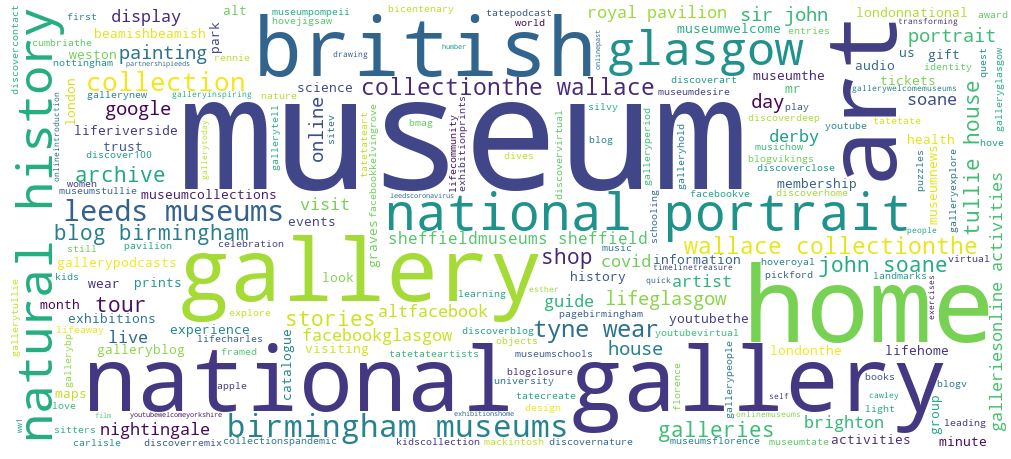
\includegraphics[width=0.6\linewidth]{images/cloud.png}
%  \centering
%   \caption{Word cloud of common keywords for digital offerings of memory institutions during COVID-19 lockdown}
% \label{fig:teaser}
% }

\maketitle
%-------------------------------------------------------------------------
\begin{abstract}
Memory institutions, including museums and heritage institutions, are a key element evidencing the past and present of societies and building their resilience in difficult times. This is particularly evident during crises, such as the outbreak of the COVID-19 pandemic. While the impact of COVID-19 dawned on people's everyday lives in early 2020, digital media consumption behaviour changed dramatically as millions of people tried to cope with the realities imposed by the lockdowns. Although a general requirement for engaging existing and new audiences of memory institutions by introducing new ways to digitally experience cultural collections has emerged over the past years; the accelerated move to online consumption due to the COVID-19 crisis significantly increased the urgency to address this gap. Thus, the research that this paper presents aims to understand how memory institutions have adapted during lockdowns by developing their digital capabilities; how these, and previous, developments ``translate" into actual digital offerings that enable to access cultural heritage resources; what are the audiences that institutions target and how their distinctive needs have been met during the COVID-19 pandemic. The research  was conducted during the lockdown period in the UK, from early spring to summer 2020, when memory institutions started to gradually re-open their physical premises to visitors. In order to acquire a more complete image of the sector's adaptation to the COVID-19 crisis, the research incorporates a comparative assessment of responses during the lockdown by collecting and analysing data from institutions both in the UK and in the United States (U.S). The contribution of the research is that it provides an in-depth understanding of the heritage sector's response to the COVID-19 crisis not only by analysing offering ``trends'' but also by examining how these offerings emerged from different institutions and whether they contributed to the overall societal needs during lockdown. \KR{offer some sentences about the conclusions of the research}

%Deploying such approach can be justified as i) both countries have a variety of museums and heritage organisations with relatively good levels of expertise and capacity in terms of digital technologies; ii) the lockdown in the UK and USA followed a similar timeline (whether this was country/state-wide or happened on a phased basis) with ``stay-at-home'' suggestions from mid-March onwards; and iii) both countries encounter similar socioeconomic challenges where heritage could make a difference or play a role.

%-------------------------------------------------------------------------
%  ACM CCS 1998
%  (see https://www.acm.org/publications/computing-classification-system/1998)
% \begin{classification} % according to https://www.acm.org/publications/computing-classification-system/1998
% \CCScat{Computer Graphics}{I.3.3}{Picture/Image Generation}{Line and curve generation}
% \end{classification}
%-------------------------------------------------------------------------
%  ACM CCS 2012
   % (see https://www.acm.org/publications/class-2012)
%The tool at \url{http://dl.acm.org/ccs.cfm} can be used to generate
% CCS codes.
%Example:
\begin{CCSXML}
<ccs2012>
   <concept>
       <concept_id>10002944.10011122.10002945</concept_id>
       <concept_desc>General and reference~Surveys and overviews</concept_desc>
       <concept_significance>500</concept_significance>
       </concept>
   <concept>
       <concept_id>10002944.10011122.10002946</concept_id>
       <concept_desc>General and reference~Reference works</concept_desc>
       <concept_significance>500</concept_significance>
       </concept>
   <concept>
       <concept_id>10010405.10010469</concept_id>
       <concept_desc>Applied computing~Arts and humanities</concept_desc>
       <concept_significance>500</concept_significance>
       </concept>
 </ccs2012>
\end{CCSXML}

\ccsdesc[500]{General and reference~Surveys and overviews}
\ccsdesc[500]{General and reference~Reference works}
\ccsdesc[500]{Applied computing~Arts and humanities}

\printccsdesc   
\end{abstract}  
%-------------------------------------------------------------------------
\section{Introduction}
\label{intro}
Memory institutions, including museums and heritage institutions, are a key element for society, especially during crises, such as the outbreak of the COVID-19 pandemic. Such institutions not only are vital for the communities they serve as research and knowledge centres, evidencing the past and present of tangible and intangible heritage; but, most importantly, form part of the communities' identity as they are an essential part of people's identity as well as a vital element for the communities by empowering people, especially in times of uncertainty such as the health crisis we experience today and its socioeconomic ramifications \cite{ICOM:2020}.

As the impact of COVID-19 on everyday lives dawned on people early in 2020, digital media consumption behaviour changed dramatically as millions of people tried to cope with the realities imposed by the lockdown. The UK reported a 29\% increase on the time spent online, and a 20\% increase of people using social media \cite{ofcom:2020}. 

Within the COVID-19 crisis, the majority of work sectors have been affected by restrictions of physical access and limited provision of services during lockdowns. As expected, the galleries, libraries, archives, and museums (GLAM) sector could not stay unaffected by the crisis. Apart from the immediate effect on institutions' workforce and finances, organisations have had to close, postpone or cancel projects, exhibitions and art programmes that they offer to their audiences. Despite these difficulties, the sector has demonstrated remarkable resilience by adapting their digital provision to allow online access to arts and culture in order to reduce isolation, improve mental health and support the educational and creative needs of diverse audiences.

The research that this paper presents was conducted during the lockdown period in the UK, from early spring to summer 2020, when memory institutions started to gradually re-open their physical premises to visitors. The aim of the research was to understand how the cultural heritage institutions have adapted during lockdowns by developing their digital cababilities; how these, and previous, developments ``translate" into actual digital offerings that enable to access cultural heritage resources; what are the audiences that institutions target and how their distinctive needs have been met during the COVID-19 pandemic. In order to acquire a more complete image of the sector's adaptation to the COVID-19 crisis, the research incorporated a comparative assessment of international responses during the lockdown by collecting and analysing data from institutions in the United States of America (USA). Deploying such approach can be justified as i) both countries have a variety of memory institutions with relatively good levels of expertise and capacity in terms of digital technologies; ii) the lockdown in the UK and USA followed a similar timeline (whether this was country/state-wide or happened on a phased basis) with ``stay-at-home'' suggestions from mid-March onwards; and iii) both countries encounter similar socioeconomic challenges where heritage could make a difference or play a role.

The research was conducted by an interdisciplinary team developing a methodology to record data through an extensive survey of digital offerings on the web and then analysing them quantitatively, while providing useful insights through qualitative analysis as well. The development of the research and its results are reported in this paper. The paper’s main contributions include: i) a unique record and useful insight into memory institutions’ digital offerings during a three-month strict lockdown period for the UK and USA; and ii) an in-depth analysis of the institutions' response to a crisis, which has the potential to inform future IT developments to keep heritage content relevant to societal needs. For instance, the analysis of data allows us to identify trends and novel ways of enabling access to heritage resources which might prove transformational in the following years.

The paper is organised as follows: Section~\ref{conrel} describes the context and related work in this area by offering an insight to other reports commissioned by other heritage organisations. Section~\ref{meth} presents the methodology which was deployed for conducting the research and capturing data. Moreover, Section~\ref{find} analyses and discusses the findings of the data which was collected. Finally, Section~\ref{disc} presents conclusions and further work.  

%-------------------------------------------------------------------------
\section{Context and related work}
\label{conrel}
As the COVID-19 pandemic started to engulf the planet in the first months of 2020, a response from governments, institutions, industries and consequently the GLAM sector was generated in order to adapt to the new reality imposed by local or nation-wide lockdowns. The following subsections describe contextual information with regards to the immediate response of major heritage stakeholders and their guidance towards museums and institutions during closures. Related work illuminating the impact of COVID-19 on the sector is also mentioned here.

\subsection{Context}
\label{con}
Memory institutions closures due to the COVID-19 pandemic started around mid-March 2020 with The Wellcome Collection in the UK and the Metropolitan Museum of Art (MET) being amongst the first ones that announced that they were shutting down \cite{McGivern2020,KendallAdams2020}. Around the same time, some of the major heritage  associations started investigating plans in order to cope with the uncertainty of closures while continuing to support communities during these difficult times. For instance, the American Alliance of Museums proposed three scenarios with different levels of impact (low, medium and high) to assist organisations to develop their own response to the crisis. These scenarios would work as the framework to manage risks in the best possible way, while supporting communities and their well-being, protecting the institutions' workforce and planning for the financial impact of the pandemic \cite{Merritt2020}.

Since then, guidance from organisations such as the Museums Association in the UK and the International Council of Museums (ICOM) would highlight similar challenges and steer the sector's adaptation by prioritising \cite{InternationalCouncilofMuseums2020a,Olorunshola2020,MuseumsAssociation2020}:
 
\begin{itemize}
\item the financial viability of heritage institutions through calls for support
\item the security of collections and the safety of staff
\item practical support of health systems by donating equipment and volunteering 
\item alternative or innovative approaches to conduct activities that cannot take place in the physical space, including new ways of working, revisiting of traditional tools and new communication channels with audiences
\item responses to societal needs and current developments, including supporting vulnerable groups such as the homeless, people suffering from dementia, children who cannot access easily education, refugees, minorities and women experiencing domestic violence
\item partnerships between institutions in the heritage sector and beyond as well as collaborations with local communities (often with emphasis on health, well-being, justice and sustainability)
\item learning from solidarity, empathy and resilience as emerged during similar situations in the past (e.g. physical catastrophes) or societal topics (e.g. human rights, conflicts and other)
\item reconsideration of accessibility standards and procedures
\item collection and documentation of the current crisis and its impact
\item reflection on the COVID-19 experience and revisiting priorities, strengths, weaknesses and practices possibly transforming the future of organisations
\item advocacy initiatives by the sector's bodies in order to secure funding and protection for organisations.
\end{itemize}

Apart, though, from setting the above priorities, heritage associations launched further guidance to reach and support audiences during the health crisis. Some of the suggested means of remote engagement were \cite{InternationalCouncilofMuseums2020,Ciecko2020,NetworkofEuropeanMuseumOrganisations20201}:

\begin{itemize}
\item online collections by offering access to digital copies or artwork (often through Open Access), exhibitions and more
  
\item online tours by deploying social media platforms, such as Facebook, Instagram Live, Pinterest curated content, Twitter threads, YouTube Live

\item podcasts to facilitate audio tours in exhibitions, discussions about the collections and analysis of interesting topics

\item blog posts and stories about a variety of collection related topics and beyond

\item social media campaigns, challenges and quizzes often with a humorous spirit by using hashtags to encourage people to share their stories (e.g. \#MuseumFromHome, \#BetweenArtandQuarantine)

\item live streams of educational activities, creative sessions, story times and more through social media and other live event platforms

\item virtual tours such as Google Arts and Culture 360-degree museum tours

\item VR/AR experiences and 3D object exploration

\end{itemize}

The above suggestions along with practical examples were proposed in order to support audiences in building resilience through informative, educational and creative activities in the period of lockdowns. Moreover, such initiatives allowed heritage institutions to continue to fulfil their societal role, with direct implications in deformalising the strong object/collection focus that many have.


\subsection{Related Work}
\label{rel}
As the coronavirus crisis rolled in, heritage institutions reacted rapidly and adapted their online presence and digital offerings. Around the same time, several funding and regulating organisations initiated efforts to record the pandemic's impact on the sector. In this way, they would be able to reflect on the institutions' response and needs in order to allocate funding and strengthen the resilience of the sector.

The Heritage Fund launched one of the first surveys in the UK in April 2020 aiming at identifying the sector's needs. Hence, institutions have been asked to respond to questions about the digital skills of their staff and the uses of digital technology they would like to explore. Intermediate results from 162 heritage organisations in the UK demonstrate that their top three priorities comprise usage of technology for a) marketing, fundraising and communication purposes; followed by b) content development; and c) community building online \cite{HeritageFund2020}.

Another research commissioned by the Art Fund (UK), gathered responses from 427 museum professionals through surveys, interviews and focus groups between April and May 2020. Findings demonstrate that 86\% of organisations have boosted their presence online. Less than half of the organisations have seen increased numbers of visitors to their websites, but there seems to be significant increase of engagement through social media. Even though there has been a rush to release a lot of content online in the first stages of the lockdown, many institutions are now developing strategic plans for their digital presence. However, in many instances there is lack of expertise and some museums are left behind in the digital world. Some of the key outcomes of the survey with respect to future digital developments point out the need to find new ways to generate income. Moreover, there is high interest in opening up collections and reaching audiences by producing new online content \cite{WaferHadley2020}.

At a European level, the Network of European Museum Organisations (NEMO) released the results of a survey that took place between March and April 2020 with responses of around 1000 professionals from museums in 48 countries. NEMO's report highlights the heavy financial impact of COVID-19 on museums; the increase of digital services as stated by four out of five museums, often by asking staff to undertake new responsibilities; the increase in online visits which is directly connected to the increase of digital offerings. As for digital offerings, museum officers reported that social media, educational material, videos and films and collection related content were amongst the most popular ones for audiences. NEMO's report concludes by emphasising the need to invest in digital services, infrastructure and digital skills' acquisition \cite{NetworkofEuropeanMuseumOrganisations20202}.

Finally, global reports from the International Council of Museums (ICOM) and the United Nations Educational Scientific and Cultural Organisation (UNESCO) evidence that the sector has been strongly impacted by financial loses with fears of permanent closures. Institutions' reaction to the crisis was fairly quick and many put efforts into their digital profile, with already existing material being the most obvious to further deploy. Furthermore, many institutions transferred scheduled programmes and events to the digital sphere; increased their digital offerings with social media content; launched quizzes, contests and challenges; organised live events, online collections, online exhibitions (often curator facilitated); and released newsletters and podcasts. The initiatives that have  been mostly introduced after the lockdown were live events and online exhibitions. Some active organisations, have emphasised the educational character of content to facilitate parents to entertain and teach children at home and also developed online participatory actions through social media. Lastly, the reports illustrate the lack of dedicated resources (staff and infrastructure) to develop the digital presence of institutions and hence a digital divide between developed and developing countries and in some instances a gender gap in accessing online content \cite{UNESCO2020,InternationalCouncilofMuseums2020b}.\KR{the paragraph below seems a similar study  to ours.. we need to be more specific on the results}

All the above reports are valuable sources of information to understand the overall impact of the COVID-19 crisis on the heritage sector. Along with more general information, the reports specify various the digital offerings' types that were prioritised while in lockdown - however they do not provide information on how this infromation was compiled (\KR{is this true???}). The novelty of the current research, though, is that it emphasises two specific countries (UK and USA that have large number of heritage institutions) to analyse deeper the digital offering ``trends''; it examines the offerings themselves as highlighted on memory institutions' websites, complementing in this way the professionals' voices; and looks at the digital offerings through the lens of audience needs and type of memory institutions to illuminate further aspects of the COVID-19 heritage response.

%-------------------------------------------------------------------------

\section{Methodology}
\label{meth}
% -> How we created the list of museums, and strategies for recording.
% Research questions:
% What  was being offered? By whom?
% Does the data demonstrate if offerings match needs that have emerged?
% The research questions which were investigated are as follows:
% 1) Which web-based digital provision was available to audiences during the UK lockdown period by UK and US museums? 
% 2) Which traditional and non-traditional audiences that this digital provision was targeting?
% 3) Which types of content museums engaged, ranging from text-based to more complex spatial-visual types of content, including Virtual Reality and panoramic images?
% 4) How museums seek financial support from audiences?
% 5) How museums kept content relevant to peoples’ challenges, including isolation, mental wellbeing and inclusivity?

%Match questions to the questions in introduction when we finalise them.
% Here we need to analyse:
% Classification of offerings under type and subtype (a table could also show what these are)
% Audiences (specific reference to Covid audiences) and what they are
% Sample selection 
% What type of analysis do we use and validity / triangulation (data triangulation: museums in two countries, national, small, civic, special theme museums \& “investigator” /analyst  triangulation: more than one researchers to collect and classify and analyse data)

The current research set out to investigate the response of the heritage sector in the UK and USA, particularly by identifying the digital offerings that were highlighted during the lockdowns. By doing this, we aim to respond to research questions that were framed as follows:

\begin{itemize}
\item Which web-based digital provision was highlighted as available to audiences during the lockdown period by UK and US memory institutions? 
\item What are the audiences that digital provision was targeting?
\item Did different types of memory institutions prioritised different offerings?
\item Which types of content memory institutions deployed, ranging from text-based to more complex spatial-visual types of content, including Virtual Reality and panoramic images?
\item What is the memory institutions' response with respect to the financial crisis as emerged from the pandemic?
\item How memory institutions kept content relevant to vulnerable communities and societal challenges, including isolation, mental well-being, accessibility and inclusivity?
\end{itemize}
%-------------------------------------------------------------------------

%\section{Data Capture}
In order to respond to the above questions, the collection of data included the survey of memory institutions' websites in the two countries. In total, we surveyed 83 memory institutions both in the UK and the US (48 in the  UK and 35 in the US). The sample included major institutions from both countries (e.g. based on visitor numbers from wikipedia) \cite{Wikipedia,Wikipediaa} plus smaller civic, historic and/or city museums. For this additional selection, we made use of the National Museums Director Council members' list in the UK \cite{nationalmuseums:2020} as well as a selection of smaller museums in different states of the US. For some memory institutions, which are aggregated under an ``umbrella'' trust, we surveyed the umbrella organisation as in most cases this presented the overall COVID response.

When surveying, researchers followed a strategy to identify what digital offering deemed as COVID-19 response, as opposed to traditional website content (e.g. top menus). In some cases, such effort proved very difficult, as many institutions re-purposed or sign-posted existing content as being COVID-19 relevant. This is not surprising given how memory institutions fulfil a role that is anyway related to the educational, well-being, and self-improving needs of communities. Thus, many organisations restructured their content to address the pandemic by creating COVID-19 ``highlights'' or ``sliders'' on their front pages. These new pages allowed users to reach a variety of relevant content instead of accessing it through the traditional website menus. The variety of COVID-19 resources in institutions was vast, and researchers followed these highlighted routes to identify which digital offerings were relevant for the survey. 

Furthermore, it was not possible to identify the impact that the digital offering had on users in terms of content visiting numbers. This happens because it is difficult to measure access to web pages without having access to museums’ web data (however this is partly evidenced by institutions' staff surveys as described in section \ref{rel}). Exceptions are the number of views on websites such as YouTube, followers in social media, or the number of downloads in sites such as SketchFab. Yet, these are difficult to directly relate to the COVID-19 response, as most content was already available before the lockdown. Instead we undertook a different approach by recording all digital offerings' corresponding URLs for later analysis. 

\KR{We still need to decide what to do with these ones}
% With these URLs, we were able to query the keywords made available on the web page titles and analyse the popularity of keywords in search queries in Google Search across various regions and languages. 

In order to offer a meaningful classification of the results, we adopted different classifications and sub-classifications including: the types of digital offerings, the type of COVID-19 audiences, the type of content, the type of memory institutions and types of donations that institutions were requesting during this period. These are described below.

\subsection{Digital offerings classification}
\label{off}
An important task that enabled us to capture meaningful data was to design an appropriate classification for digital offerings. This classification had to facilitate us to record as accurately as possible the purpose of the content offered to visitors during the COVID-19 lockdown period. As mentioned previously, the majority of content was not specific to COVID-19 related topics. Hence, the classification was generic to deal with a variety of offerings by memory institutions. Table~\ref{tab:digoffer} shows the classification, which categorises offerings into seven types: collection, virtual visit, learning, home activities, events, funding and communication. Inevitably, there are certain overlaps between different types, as access to a collection could enable learning or be a home activity. However, we categorised digital offerings %according to how the content was being presented using a variety of keywords to highlight its purpose.
under the most obvious type, while deploying a set of subtypes that could further help the classification process.

Table~\ref{tab:digoffer} also demonstrates the subtypes we designed to further classify digital offerings. This was particularly important for understanding the types of access to collections or exhibitions being offered, the types of events memory institutions organised, the types of communication strategies they used during this period, types of home activities and more. For instance, subtypes of the ``Collection'' type digital offering could include: free database exploration, guided exploration, collection related resources, 3D collection, image database/resources as well as collecting content. The latter was particularly interesting as some memory institutions set to actively collect digital content or objects from the public during the lockdown period to document the COVID-19 impact to communities.

\begin{table}
\begin{tabular}
{ | l | l | }
    \hline
    \textbf{Digital Offering Type}  & \textbf{Subtype}  \\
    \hline
  \multirow{6}{*}{Collection} & Free database exploration  \\
&  Guided exploration  \\
&  Collection related resources \\
&  3D collection \\
&  Images database/resources \\
&  Collecting content \\
    \hline
 \multirow{2}{*}{Virtual visit} & Gallery tour  \\
&  Audio tour  \\
    \hline
 Learning & Educational material  \\
    \hline
 \multirow{2}{*}{Home activities} & Creative activities \\
&  Wellbeing activities  \\
    \hline
 \multirow{4}{*}{Events} & Festival\\
&  Live event \\
&  Other \\
&  Competition \\
    \hline
 Funding & comercial venture \\
    \hline
 \multirow{12}{*}{Communication} & COVID-19 communication \\
& Podcast \\
& Blog/articles' section \\
& Social media  \\
& Videos \\
& Student/artist resources \\
& Racism related \\
& Practical info \\
& Digital publications \\
& Practical info \\
& Music lists \\
& Other \\
    \hline
\end{tabular}
\caption{\label{tab:digoffer}Digital offering types and subtypes used in the survey}
\end{table}

\subsection{COVID-19 audiences}
\label{covaud}
As a means to understand which were the audiences that the digital offerings from heritage institutions targeted, we deployed a segmentation of COVID-19 relevant audiences. Although it might have been possible to adapt existing segmentation as used by institutions \cite{Drot19}, we adopted Jones' \cite{Audiences2020} COVID-19 audience segmentation. This segmentation takes into account how digital offerings of memory institutions might fulfil emotional needs of people affected by the pandemic. As such, the classification distinguishes between the needs of three groups of audiences, which are then further classified into distinctive types: 

\begin{itemize}
	\item \textit{Audiences seeking learning support}: traditional audience of memory institutions where emphasis is on helping with acquiring knowledge for formal and informal education, including supporting with online learning, reflection and thinking. Examples include teachers, eager learners, parents doing homeschooling.
	\item \textit{Audiences seeking emotional support and entertainment}: Emphasis is on those who are seeking content or activities (e.g. arts and crafts activities), which might provide additional benefits. These benefits include relaxation, well-being, and support to process what is happening around the world as well as in their personal lives. Examples include bored people, stressed out/scared, workers (both working at home and those having to go to their workplace), lonely people and those wanting to help others. 
	\item \textit{Stakeholders who wish to keep involved}: Emphasis is on those audiences which are critical for the operation of an organisation or who depend on it. They seek to understand how the pandemic is affecting the organisation, themselves and how they can offer support in this process. These audiences include internal audiences, museum constituencies (e.g. core audiences for content), museum members or donors, and the local community.
\end{itemize}


\subsection{Types of content}
\label{typ}
To further understand what the digital offerings consist of, the survey recorded a description for every offering as well as the type of content. Even though most web pages comprise text and image elements, the survey included information about more complex data types, such as video (including live video stream), audio, interactive games and activities, 3D objects explorations, 360º virtual tours and interactive panoramas/VR/AR type experiences.
% here I changed the sequence of offerings as the ones analysed below probably refer to VR, AR and panoramas etc and visual content
The visual types of content are of particular interest, as they allow audiences to engage more actively with the digital content. Hence, they enable people to explore a collection or an exhibition's physical space by providing images of the collection, interactive panoramic tours, behind the scenes audiovisual material, and virtual galleries' visit. Besides being a popular type of content, visual content has some advantages for audiences, such as being more inclusive to multiple understandings and interpretations, as well as overcoming communication barriers, such as language and attention barriers. However, it can also be less accessible for those with disabilities if the content has not been designed appropriately.

\subsection{Sample selection}
\nllabel{sam}
The survey included a variety of memory institution types as illustrated in Figure~\ref{fig:MType}. Some institutions were more difficult to categorise due to the variety or particularity of their collections. In this case we opted for the most prevalent type or grouped them under one category (e.g. maritime/military museums). The data recorded for each museum also included the city and country where the museum was located, as well as a Wikidata code so that more information could be retrieved during the analysis phase.

\subsection{Funding and donations}
\label{fund}
Given the severe financial impact of COVID-19 on heritage institutions as also highlighted by major sector organisations (see section \ref{conrel}), the survey recorded data regarding funding and calls for donations. Thus, although many institutions normally request for donations, the survey specifically recorded calls for donations in relation to the COVID-19 crisis (e.g. emphasised by messages about the current crisis and urgent need for support). The overall data that were recorded about funding included i) calls for donations emphasising (or not)  COVID-19, ii) calls to support through other means, such as shop purchases, memberships or gifts; and iii) no existence of specific calls.

\subsection{Other data}
\label{other}

Beside the previously described types of information, data was also recorded - when available - regarding the author and date of creation of the digital offering, its URL and any additional comments which were worth recording and could facilitate a further qualitative analysis of findings.

All data were recorded from April the 23$^{rd}$  2020, only one month after the UK went into lockdown, until the 31$^{st}$ of July 2020, a few weeks after museums and galleries were allowed to reopen to the public in the UK. Both data collection and analysis was realised by an interdisciplinary team of researchers, providing in this way further validity due to ``investigator'' and analyst triangulation for the research.

The following section presents and analyses the resulting data. 
 
%-------------------------------------------------------------------------

\section{Findings of Data Survey}
\label{find}
The analysis of data allowed us to explore in detail the digital offerings of memory institutions during the COVID-19 lockdown period in order to respond to the research questions. To recap, these questions are related to: 1) the types of digital offerings which were available to audiences; 2) the types of audiences these offerings targeted; 3) the offerings that different museum types prioritised; 4) the nature of the offerings' content; 5) the financial support sought by museums during the crisis; and 6) exploring how the digital offerings matched needs that emerged during the COVID-19 pandemic in particular with regards to vulnerable communities and societal challenges, including isolation, mental well-being and inclusivity. 

A total of 922 digital offerings were recorded as providing relevant content for the COVID-19 crisis amongst all memory institutions. This includes a total of 515 digital offerings in the UK, and 407 digital offerings in the US; with an average of 11 digital offerings per memory institution. We reiterate that not all of this content was newly created, but could have been restructured and highlighted as relevant to the perceived needs of audiences during the lockdowns. 

The following subsections present the analysis of data regarding the surveyed memory institutions, types of offerings, audiences, financial issues and all topics as they emerge from the research questions.

\subsection{Memory institutions surveyed}
\label{inst}
As Figure~\ref{fig:MType} illustrates the survey included a mixture of institutions ranging from History/Historic house or place (18\%), Art (14\%), Art and History (12\%), Polythematic (10\%), Museum Trust (8\%), Special Theme (8\%), Science (8\%), Maritime/Military (8\%), Natural History (7\%), and Library/Archive (5\%). Within these variety of institutions, there are representatives of different types of collections, galleries, exhibitions and historic environments; all of which can be experienced through a variety of digital offerings. 


\begin{figure}[h]
  \centering
  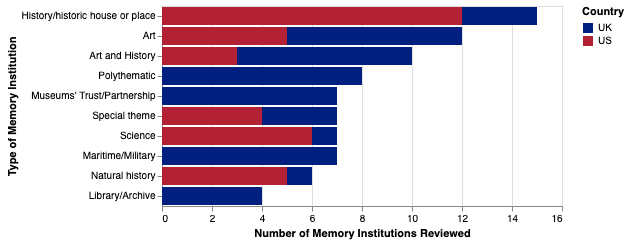
\includegraphics[width=\linewidth]{images/museumtype.png}
  % replacing the above command with the one below will explicitly set
  % the bounding box of the PS figure to the rectangle (xl,yl),(xh,yh).
  % It will also prevent LaTeX from reading the PS file to determine
  % the bounding box (i.e., it will speed up the compilation process)
  % 
\includegraphics[width=.95\linewidth, bb=39 696 126 756]{sampleFig}
  %
  % \parbox[t]{.9\columnwidth}{\relax
  %          For all figures please keep in mind that you \textbf{must not}
  %          use images with transparent background! 
  %          }
  %
  \caption{\label{fig:MType}
           Types of memory institutions surveyed}
\end{figure}

Moreover, Figure~\ref{fig:typeofferings} presents the number of digital offerings recorded for each type of memory institution. In average, History/Historic houses provided 10 offerings, Art institutions provided 12 offerings, Art and history institutions provided 13 offerings, Polythematic institutions provided 14 offerings, Museum Trusts provided 9 offerings, Special Theme institutions provided 10 offerings, Science institutions provided 11 offerings, Maritime/Military institutions provided 11 offerings, Natural History institutions provided 12 and Library/Archive institutions provided 12 offerings. 

\begin{figure}[h]
  \centering
  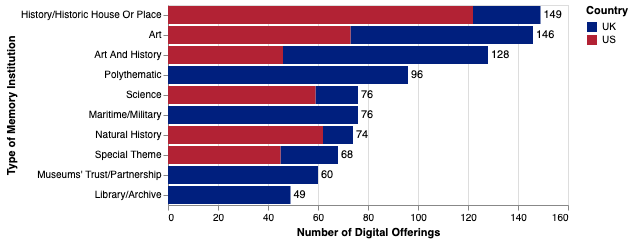
\includegraphics[width=\linewidth]{images/typesoffering.png}
  \caption{\label{fig:typeofferings}
           Number of digital offerings provided by different types of institutions}
\end{figure}



% 922 total
%515 UK
%407 US

\subsection{Digital offerings}
\label{dig}
With regards to types of digital offerings, Figure~\ref{fig:TypeComparisonUKUS} and Figure~\ref{fig:SubTypeComparisonUKUS} show a comparison between the number of digital offerings both in the UK and the U.S. classified according to their type and subtype. Digital offerings of \emph{Collection} (28\%) and \emph{Communication} (43\%) type were the most popular in both countries. For the UK, \emph{Collection} type of digital offerings represented a 29\%; while \emph{Communication} type of digital offerings represented a 42\% of the total offering for the UK. For the U.S., \emph{Collection} type of digital offerings represented a 25\%; while \emph{Communication} type of digital offerings represented a 45\% of the total offering for the U.S. 


On the lower end, virtual visits represented only a 2\% both for the UK and the U.S. making it the lower type of digital offering for both countries. It is interesting the fact there  were so few virtual visits being offered, despite the fact audiences could not physically visit memory institutions. Probably, the biggest barrier for this was the lack of content of such experiences. Some examples of virtual visits which were provided include last minute videos of the curator of Michelangelo's exhibition at the Getty Museum in empty rooms before the museum's closure \cite{getty2020}.  


For different subtypes of offerings, there are few significant differences between the countries with most offering showing a percentage difference amongst the countries of less than 3\%. The only exceptions are \emph{Guided exploration} digital offerings, which are 12\% of the offering in the UK and 8\% of the offering in the U.S; \emph{Live events} digital offerings which are 3\% of the offerings in the UK and 6\% of the offerings in the U.S.; and \emph{Others} which are 12\% of the offering in the UK and 9\% of the offerings in the U.S. The latter one refers to \KR{what is recorded under this type}. 
 
\begin{figure*}[h]
  \centering
  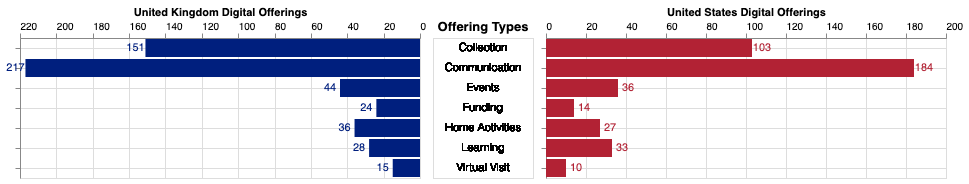
\includegraphics[width=\linewidth]{images/typecomparison.png}
  \caption{\label{fig:TypeComparisonUKUS}
           Comparison of offering types between US and UK}
\end{figure*}
\begin{figure*}[h]
  \centering
  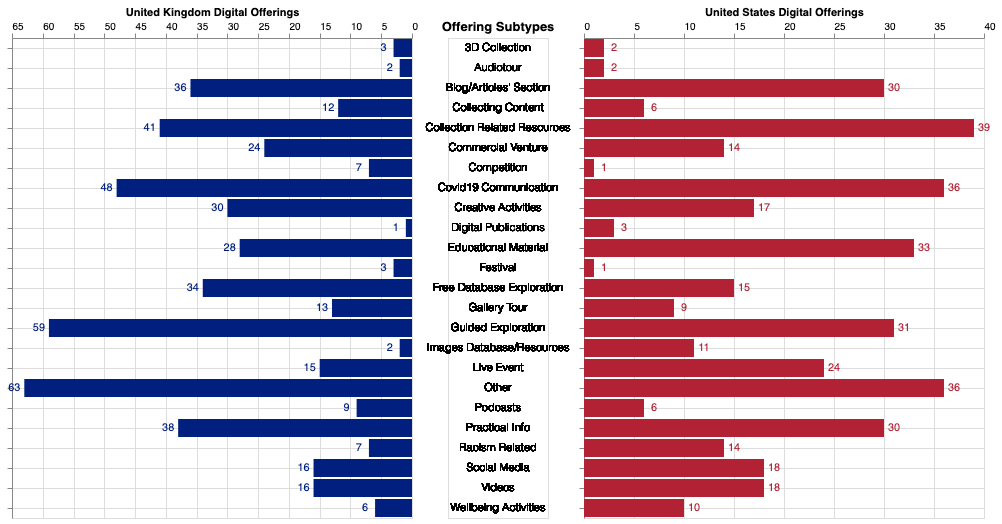
\includegraphics[width=\linewidth]{images/subtypecomparison.png}
  \caption{\label{fig:SubTypeComparisonUKUS}
           Comparison of offering subtypes between US and UK}
\end{figure*}

 
% \begin{figure}[h]
%   \centering
%   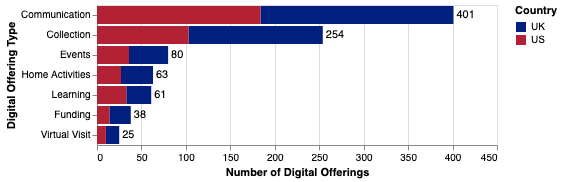
\includegraphics[width=\linewidth]{images/digitalTypes.png}
%   \caption{\label{fig:DigOffType}
%            Number of digital offerings provided for each type of digital offering during the COVID-19 period}
% \end{figure}

% 60 digital offerings amongst 7 institutions, with an average of 8 offerings), given their overall representation in the sample  

% 49 /

% 60 /


Furthermore, Figure~\ref{fig:MTypeOfferings} cross-relates the number of offerings types with the different types of memory institutions which provided them. 

\begin{figure}[h]
  \centering
  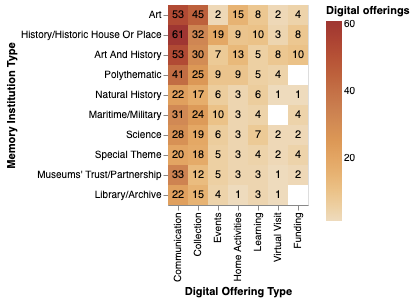
\includegraphics[width=\linewidth]{images/museumoffering.png}
  \caption{\label{fig:MTypeOfferings}
           Digital offerings provided by different types of memory institutions and under different digital offering types}
\end{figure}

Both Figure~\ref{fig:DigOffType} and Figures~\ref{fig:MTypeOfferings} illustrates that digital offerings both for providing access to memory institutions' collection and communicating with audiences were the most popular both in the UK and the US. This demonstrates the value which memory institutions place on enabling access to collection content in terms of fulfilling their remit throughout the lockdown period. In addition, memory institutions actively sought to keep in contact with audiences. This also confirms that memory institutions responded well to advice to keep communication with audiences via alternative channels of communication through digital tools and platforms. 




The less explored type of digital offering relates to \emph{Funding}, with only 4\% of the digital offerings related to this aspect. This is somehow surprising given how the lack of funding might affect memory institutions post-COVID-19. Although, there is also an element of lack of digital offerings or business models which can allow memory institutions to generate additional funding. Interesting examples were found regarding digital offerings which are commercial ventures, includes recipe boxes to buy with all the ingredients and instructions to prepare food at home offered by Birmingham Museum \& Art Gallery; or genealogy search services offered by the Statue of Liberty-Ellis Island Foundation which provided research to trace family history/arrival to America by the institution research staff. Also, there were some museums which generated income by organising ticketed live events, such as the online science camp for pupils organised by California Science Centre.





% 679 eager learners
% 417 teachers
% 19 grieving - 2%
% 12 PWTHO - 2%
% 922 total

\subsection{Audiences}
\label{aud}

Figures~\ref{fig:MTypeAudiences} presents the offerings targeted to specific audiences by each type of memory institution both in the UK and the US. The data illustrates the strong emphasis on memory institutions addressing educational needs of audiences during the pandemic, with a strong focus on audiences who seek opportunities to gain new knowledge, such as teachers and higher education academics, as well as learners in both countries. For instance, the data highlights how \emph{Eager learners} were the most dominant type of audiences with 74\% of digital offerings. Audiences created by COVID-19, such as those grieving (2\%) or wanting to help others, e.g. carers, (2\%) where those less directly targeted by offerings.

\begin{figure}[h]
  \centering
  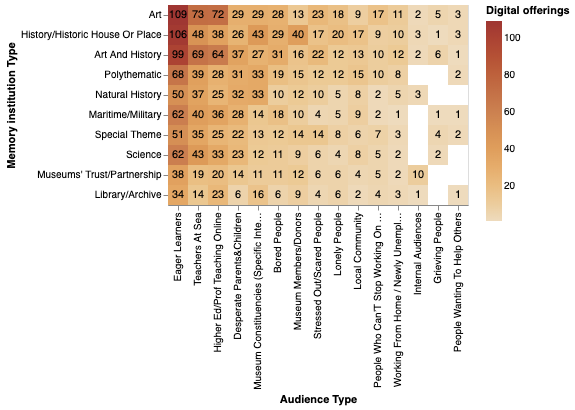
\includegraphics[width=\linewidth]{images/audiencesboth.png}
  \caption{\label{fig:MTypeAudiences}
           Digital offerings provided by different types of memory institutions and targeted to different audience types}
\end{figure}


% Table~ref

% \begin{figure}[h]
%   \centering
%   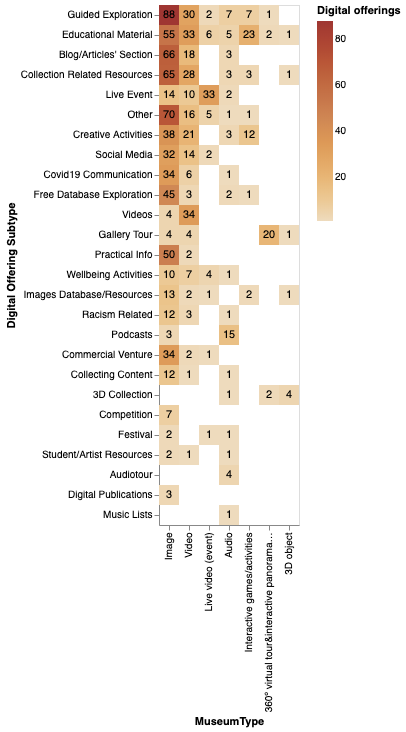
\includegraphics[width=\linewidth]{images/typescontent.png}
%   % replacing the above command with the one below will explicitly set
%   % the bounding box of the PS figure to the rectangle (xl,yl),(xh,yh).
%   % It will also prevent LaTeX from reading the PS file to determine
%   % the bounding box (i.e., it will speed up the compilation process)
%   % 
\includegraphics[width=.95\linewidth, bb=39 696 126 756]{sampleFig}
%   % %
%   % \parbox[t]{.9\columnwidth}{\relax
%   %          For all figures please keep in mind that you \textbf{must not}
%   %          use images with transparent background! 
%   %          }
%   %
%   \caption{\label{fig:MTypeAudiences}
%            Types of Content made available by institutions both in the UK and the US.}
% \end{figure}

%146/922 for first group
%588/922 for second group
%285/922 for third group



Moreover, Figure~\ref{fig:Subtypeaudiences} shows the digital offerings for the three distinct groups of audiences: emotional needs  \emph{(left)}, educational needs \emph{centre}, stakeholder involvement needs \emph{(right)}. These Figures show that the three most popular digital offerings for audiences seeking emotional support included social media, live events and creative activities. These offerings represent a 16\% of the total digital offering recorded. Those seeking support with informal and formal learning received guided exploration of the collection, educational material and collection related resources as top digital offerings, which is a 64\% of the total. Stakeholders of memory institutions were targeted mainly by COVID-19 communication, blog and articles, and practical information. This represents a 31\% of the total offering.

\begin{figure*}[h]
  \centering
  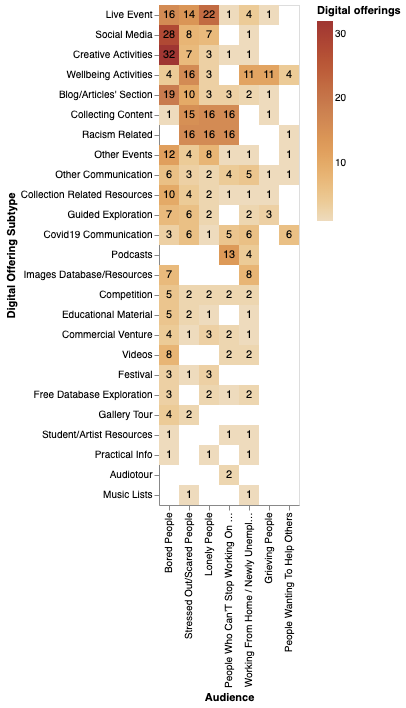
\includegraphics[width=.34\linewidth]{images/emotionalneeds.png}
  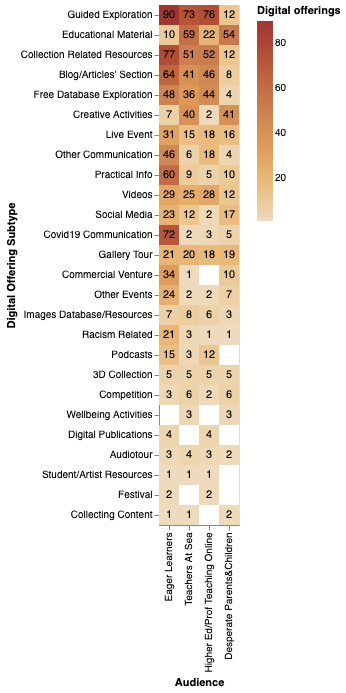
\includegraphics[width=.29\linewidth]{images/educationneeds.png}
  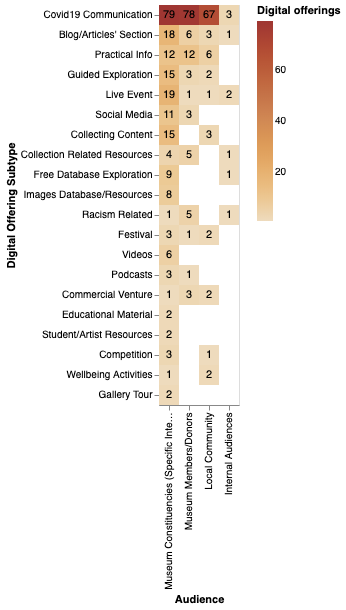
\includegraphics[width=.32\linewidth]{images/internalneeds.png}
  \caption{\label{fig:Subtypeaudiences} Audiences-based digital offerings classified according to the primordial audiences needs: emotional needs  \emph{(left)}, educational needs \emph{centre}, stakeholder involvement needs \emph{right}}

\end{figure*}


The analysis of the data related to audiences suggests that most memory institutions focused primordially on traditional audiences;  rather than those newly created during the COVID-19 pandemic, including lonely or grieving people. It also confirms that institutions might have re-purposed material, already available, which support core aims of these institutions as knowledge providers for audiences. As a result, it is noted a lack of digital offerings focusing on tackling specific well-being and emotional needs of these type of audiences. Some interesting example  of this  type of offerings includes physical activity packs which were offered by the Exeter Royal Albert Memorial Museum \& Art Gallery to shielded, vulnerable and isolated people in the city to help ease lockdown boredom \cite{ex2020}; as well as a ``Cultural First Aid kit'', developed by Manchester Museum, focusing on well-being for people in hospitals and care centres \cite{man2020}. 

\color{red}until here checked \color{black}








 subtypes of digital offerings for the \emph{Collection} type of digital offering. The total of offerings for guided exploration represented the largest amount. Of interest are those collection and resources which were addressing  societal concerns during the COVID-19 lockdown period, including the Black Live Matters activism movement in the UK and the US. \KR{Do we have an interesting example of resources offered?}

%For instance, the San Francisco Museum of Modern Art(SFMOMA) statement about artists who have recalled their work from the museum's website as a response to the Black Lives Matter protests.
% \begin{figure}[h]
%   \centering
%   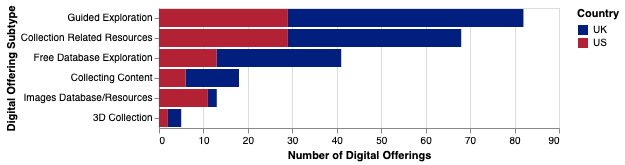
\includegraphics[width=\linewidth]{images/collection.png}
%   \caption{\label{fig:Collection}
%            Subtypes of digital offerings of Collection type }
% \end{figure}




\color{red}To answer:
Which museums target groups that need support through wellbeing activities
How many museums collected content 
\color{black}

However, there is less evidence on how these digital provision might have reached or engaged with some of the groups identified under risk, such as women at risk of domestic violence, children with difficult access to education, migrants, refugees, unemployed, health workers and minorities experiencing increased discrimination and xenophobia. 
% \begin{figure}[h]
%   \centering
%   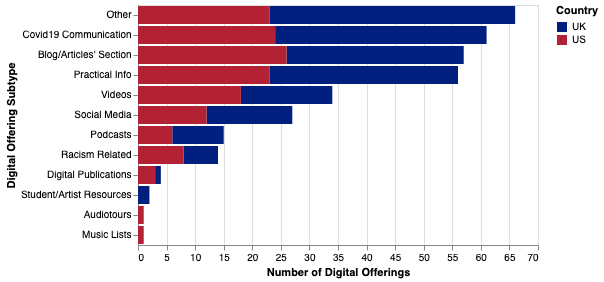
\includegraphics[width=\linewidth]{images/communication.png}
%   \caption{\label{fig:DigOffType2}
%            Subtypes of digital offerings of Commuincation type}
% \end{figure}

\color{red}To answer: Data  categorised  as  type of museum - do focus on wellbeing happening by certain types of museums?\color{black}

\begin{figure}[h]
  \centering
  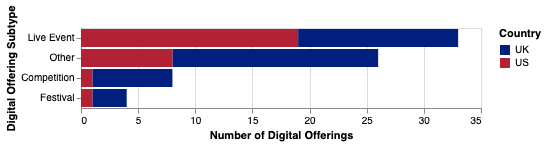
\includegraphics[width=\linewidth]{images/event.png}
  \caption{\label{fig:DigOffType3} 
           Subtypes of digital offerings of Event type}
\end{figure}

\subsection{Audiences targeted by digital provision}
\label{targ}
\color{red}To answer: Which audience is mostly targeted for the overall provision?\color{black}

% \begin{figure}[h]
%   \centering
%   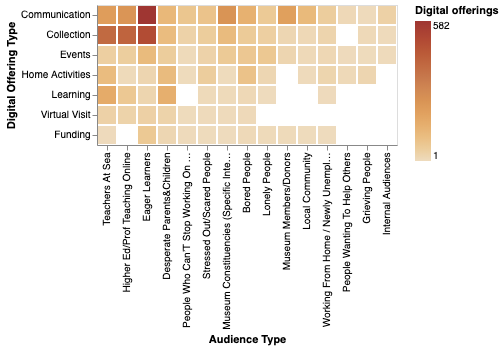
\includegraphics[width=\linewidth]{images/typeaudience.png}
%   \caption{\label{fig:DigOffType4}
%            Types of digital offerings targetted to different audiences
%            }
% \end{figure}

% \begin{figure}[h]
%   \centering
%   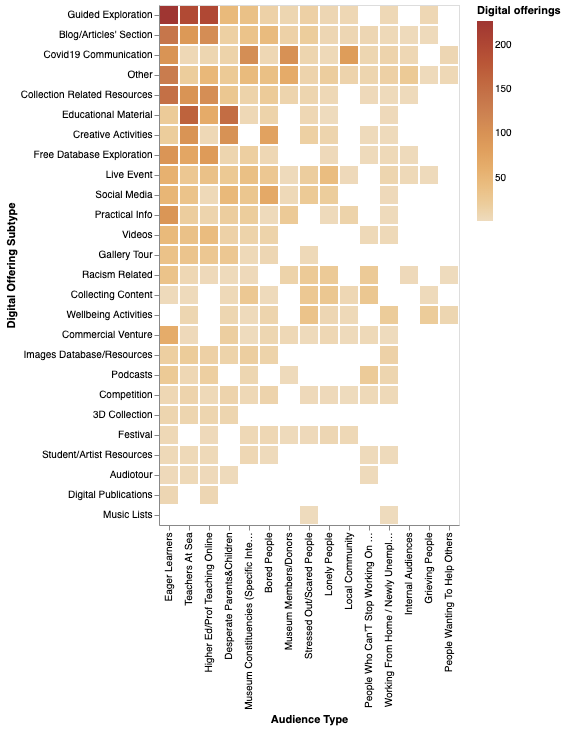
\includegraphics[width=\linewidth]{images/subtypeaudience.png}
%   \caption{\label{fig:DigOffType5}
%                       Types of digital offerings targetted to different audiences}

% \end{figure}

\noindent \textbf{Content for audiences}
\color{red}To answer: Which is the strongest/more popular format ?\color{black}


% \begin{figure}[h]
%   \centering
%   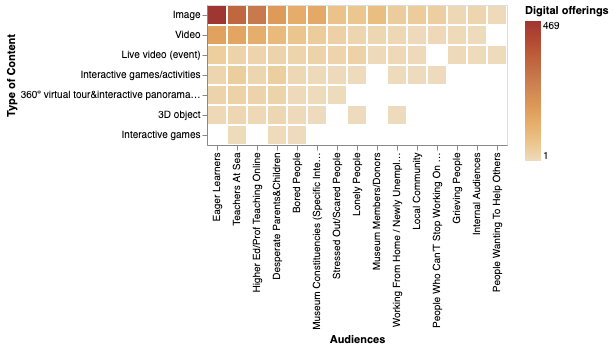
\includegraphics[width=\linewidth]{images/contentaudience.png}
%   \caption{\label{fig:DigOffType6}
%                       Types of content provided to different audiences}

% \end{figure}

\subsection{Funding and donations}
\label{don}
\color{red}To answer: What do data show about donation campaigns?\color{black}



\subsection{Interesting offerings}
\label{int}
Demonstrate some of the novelties that have emerged (look at section 3 of my document and add to categories below)
Also: 
Curators’ view and tours in exhibitions to give a “personal touch” (plus last minute “emergency” tours before closure)
Covid related content collection (to document the health crisis)
Monetizing digital offerings (income generating)
Connection to other sites and cultural institutions (solidarity)
Well being, mental health focus, mention the very limited examples that offer physical offerings for those  that do not have access to the digital provision.
Surveys about the future of digital offerings and reopening
Decolonisation, Black lives matter
Which digital offering request for payment? (I think this cannot be added here, but rather in the section of “special offerings”)

\section{Discussion and conclusions}
\label{disc}
Identified gaps:
More training/skills are required to fulfill the novel digital requirements (digital literacy within the house). Freelancers have been amongst the first groups who stopped working for museums and there is no financial capacity to pay for freelancers' work (even though these were often assisting with digital work before the covid crisis). In order to adapt to the situation in house staff have had to take on new responsibilities. Also, digital inequality between big and smaller/rural museums is evident in reports and funding for digital activities is minimum (see section 7 of my document).
Marketing opportunities  - how can museums produce revenue from digital offerings. How people have monetised digital offerings? (look at Money list article)
Lack of agreed methods and metrics to measure digital engagement (mention relevant research and efforts -e.g. The audience agency- but there is no consensus).
Future development:
How can this content have a legacy beyond the lockdown and how the priorities of the sector might change (focus on digital instead of physical, communication between staff, more flexible working, diversity and inclusion because of flexible working, use of external spaces for exhibitions etc?)
How local strategies can be developed to build resilience especially for older people (at home or in care homes), shielding people, people with mental health issues, grieving communities etc (mention access to physical activities too). 
How digital can help not only audiences, but the way the museums work and function under the new normal? (Contactless interactives; Own mobile device tour apps; Visitor flow management; Virtual tours and the virtual museum.)
Issues that have have not been adequately addressed during the crisis:
Services/offerings for disabled audiences (could also make reference to our work with blind audiences an 3d prints that could be offered as a “print on demand” service in a similar way that museums offer prints of works of art). Generally lack of special provision (physical objects, sign language, look at Vocal Eyes newsletters)
Diversity and decolonisation through/for the digital provision by addressing the sparsity of current efforts (maybe mention the SFMOMA examples here as well).

-> any discussion regarding what future work is of interest, and conclusions
->  how things might evolve
Future work will include to develop a better  understanding on how audiences engaged with this type of content  , and the impact that it is having on audiences. 





% %%%
% %%% Figure 1
% %%%
% \begin{figure}[htb]
%   \centering
%   % the following command controls the width of the embedded PS file
%   % (relative to the width of the current column)
%   
\includegraphics[width=.8\linewidth]{sampleFig}
%   % replacing the above command with the one below will explicitly set
%   % the bounding box of the PS figure to the rectangle (xl,yl),(xh,yh).
%   % It will also prevent LaTeX from reading the PS file to determine
%   % the bounding box (i.e., it will speed up the compilation process)
%   % 
\includegraphics[width=.95\linewidth, bb=39 696 126 756]{sampleFig}
%   %
%   \parbox[t]{.9\columnwidth}{\relax
%            For all figures please keep in mind that you \textbf{must not}
%            use images with transparent background! 
%            }
%   %
%   \caption{\label{fig:firstExample}
%            Here is a sample figure.}
% \end{figure}


%-------------------------------------------------------------------------
% bibtex
\bibliographystyle{eg-alpha-doi}  
\bibliography{egbibsample}        

% biblatex with biber
% \printbibliography                

%-------------------------------------------------------------------------


\end{document}

